% IncludeFile style
% Typical usage (all UPPERCASE items are optional):
%       \input includeFile
%       \begin{document}
%       \MYTITLE{Title of document, e.g., Lab 1\\Due ...}
%       \MYHEADERS{short title}{other running head, e.g., due date}
%       \PURPOSE{Description of purpose}
%       \SUMMARY{Very short overview of assignment}
%       \DETAILS{Detailed description}
%         \SUBHEAD{if needed} ...
%         \SUBHEAD{if needed} ...
%          ...
%       \HANDIN{What to hand in and how}
%       \begin{checklist}
%       \item ...
%       \end{checklist}
% There is no need to include a "\documentstyle."
% However, there should be an "\end{document}."
%
%===========================================================
\documentclass[11pt,twoside,titlepage]{article}
%%NEED TO ADD epsf!!
\usepackage{threeparttop}
\usepackage{graphicx}
\usepackage{latexsym}
\usepackage{color}
\usepackage{listings}
\usepackage{fancyvrb}
%\usepackage{pgf,pgfarrows,pgfnodes,pgfautomata,pgfheaps,pgfshade}
\usepackage{tikz}
\usepackage[normalem]{ulem}
\tikzset{
    %Define standard arrow tip
%    >=stealth',
    %Define style for boxes
    oval/.style={
           rectangle,
           rounded corners,
           draw=black, very thick,
           text width=6.5em,
           minimum height=2em,
           text centered},
    % Define arrow style
    arr/.style={
           ->,
           thick,
           shorten <=2pt,
           shorten >=2pt,}
}
\usepackage[noend]{algorithmic}
\usepackage[noend]{algorithm}
\newcommand{\bfor}{{\bf for\ }}
\newcommand{\bthen}{{\bf then\ }}
\newcommand{\bwhile}{{\bf while\ }}
\newcommand{\btrue}{{\bf true\ }}
\newcommand{\bfalse}{{\bf false\ }}
\newcommand{\bto}{{\bf to\ }}
\newcommand{\bdo}{{\bf do\ }}
\newcommand{\bif}{{\bf if\ }}
\newcommand{\belse}{{\bf else\ }}
\newcommand{\band}{{\bf and\ }}
\newcommand{\breturn}{{\bf return\ }}
\newcommand{\mod}{{\rm mod}}
\renewcommand{\algorithmiccomment}[1]{$\rhd$ #1}
\newenvironment{checklist}{\par\noindent\hspace{-.25in}{\bf Checklist:}\renewcommand{\labelitemi}{$\Box$}%
\begin{itemize}}{\end{itemize}}
\pagestyle{threepartheadings}
\usepackage{url}
\usepackage{wrapfig}
% removing the standard hyperref to avoid the horrible boxes
%\usepackage{hyperref}
\usepackage[hidelinks]{hyperref}
% added in the dtklogos for the bibtex formatting
%\usepackage{dtklogos}
%=========================
% One-inch margins everywhere
%=========================
\setlength{\topmargin}{0in}
\setlength{\textheight}{8.5in}
\setlength{\oddsidemargin}{0in}
\setlength{\evensidemargin}{0in}
\setlength{\textwidth}{6.5in}
%===============================
%===============================
% Macro for document title:
%===============================
\newcommand{\MYTITLE}[1]%
   {\begin{center}
     \begin{center}
     \bf
     CMPSC 300\\Bioinformatics\\
     Fall 2019 
     \medskip
     \end{center}
     \bf
     #1
     \end{center}
}
%================================
% Macro for headings:
%================================
\newcommand{\MYHEADERS}[3]%
   {\lhead{#1}
    \rhead{#2}

%    \def \dateofhandout {January 17, 2017}
%    \lfoot{\sc Handed out on \dateofhandout}

    \def \dateofhandout {#3}
    \lfoot{\sc \dateofhandout}

   }

%================================
% Macro for bold italic:
%================================
\newcommand{\bit}[1]{{\textit{\textbf{#1}}}}

%=========================
% Non-zero paragraph skips.
%=========================
\setlength{\parskip}{1ex}

%=========================
% Create various environments:
%=========================
\newcommand{\PURPOSE}{\par\noindent\hspace{-.25in}{\bf Purpose:\ }}
\newcommand{\SUMMARY}{\par\noindent\hspace{-.25in}{\bf Summary:\ }}
\newcommand{\DETAILS}{\par\noindent\hspace{-.25in}{\bf Details:\ }}
\newcommand{\HANDIN}{\par\noindent\hspace{-.25in}{\bf Hand in:\ }}
\newcommand{\SUBHEAD}[1]{\bigskip\par\noindent\hspace{-.1in}{\sc #1}\\}
%\newenvironment{CHECKLIST}{\begin{itemize}}{\end{itemize}}

\begin{document}

\MYTITLE{Project Assignment}
\MYHEADERS{}{\color{red} See due dates for individual parts\color{black}}{Handed out: 4$^{th}$ November 2019}
% Due: 9$^{th}$ Sept
\flushleft

\begin{figure}[ht!]
	\begin{center}
	 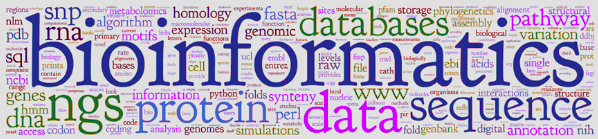
\includegraphics[scale=.7]{graphics/bioinfo.png}
	\end{center}
	\caption{Bioinformatics contains many different types of research.}
	\label{fig:bioinfo}
\end{figure}


\vspace*{-.1in}
\section*{GitHub Starter Link for Groups}
\vspace*{-.1in}
\begin{center}
\color{red}STOP! STOP!\\ Not everyone will be clicking this link at this time!\\ Only the team leader will be clicking the link to create the repository!!\\ \url{https://classroom.github.com/g/7h96fjD7}\color{black}
\end{center}

\subsection*{Creating your repository}
%To use this link, please follow the steps below.

We will use a group assignment functionality
of GitHub Classroom for this assignment. For group assignments \textbf{only one person will be creating the team while the other team members will join that team.} Please form a team of \textbf{no more than three people} and select one person to create the repository.


The selected person of the team should go into the link of the assignment sheet. Copy this link and paste it into your web browser. Now, you should accept the assignment and create a new team with a unique and descriptive team name (under the field marked, ``Create a new team.'')

Now the other members of the team can click on the assignment link and select their team from the list under ``Join an Existing Team.'' When other team members join their group in GitHub Classroom, a team is created in our GitHub organization. Every team member will be able to push and pull to their team’s repository. 

\textbf{Please work in groups and leave no-one out of the loop}: Working in groups is one of the best ways to add focus to your project and to develop ideas (by brainstorming.) This focus can only happen when you include everyone in your group. Please do not leave any group member behind in your thinking and planning of your project.
%Unless you provide the instructor with documentation of the extenuating circumstances that you are facing it will be expected that your work will be in a group setting.



To push your changes, you can use the following commands to add a single file, you must be in the directory where the file is located (or add the path to the file in the command):
	\begin{itemize}
		\item {\tt git commit <nameOfFile> -m ``Your notes about commit here''}
		\item {\tt git push}
	\end{itemize}
	Alternatively, you can use the following commands to add multiple files from your repository:
		\begin{itemize}
		\item {\tt git add -A}
		\item {\tt git commit -m ``Your notes about commit here''}
		\item {\tt git push}
	\end{itemize}
%\end{itemize}

\vspace*{-.1in}
\subsection*{Reading Assignment}
\vspace*{-.1in}
To help you work, please read the covered chapters from the course book, consult the week's slides and your class notes. You can also find useful information in the Python community by performing online research for programming help. Please take some time to gain experience with using Markdown to complete your writing assessments. \textbf{Your written deliverables (are to be written in Markdown.} 

See \emph{Mastering Markdown}  \url{https://guides.github.com/features/mastering-markdown/} for more details about Markdown. Another good reference may be found at: \url{https://markdown-it.github.io/}. 

%%%

Be sure to read the {\tt README.md} file in the GitHub Classroom repository for instructions on how to complete your first assignment.

\vspace*{-.1in}
\subsection*{Summary}
\vspace*{-.1in}

Throughout the semester, you have studied many of the concepts listed in Figure \ref{fig:bioinfo}, and have also used various computational tools such as alignment and BLAST to explore a number of biological phenomena. The final project invites you to explore, in greater detail, a real-world application of bioinformatics. You will research in more depth a real-world bioinformatics project that is interesting to you and carry out a computational investigation through the use, implementation, testing, and evaluation of different types of software.

\noindent For your final project, you can work individually or in groups of two or three. If you decide to work in a group, each member of the group will be evaluated separately based on his or her contributions to the project. This evaluation will be determined largely from the feedback of the group members.Please be sure to include all names of your group members in each deliverable that you submit. Remember, groups are up to three (3) members. 

\vspace*{-.1in}
\subsection*{Assignment Specifications}
\vspace*{-.1in}

For the project assignment you may choose a biological research question that is of the most interest to you and can be investigated through computational technique(s). Pick something realistic and useful, for example, you can choose specific question(s) related to the topics we discussed during the first week of the course. You may use anything and everything we have learned (or will learn) in class and also you should research additional resources beyond of what we discussed in class. You may also extend any of the programs or concepts we have developed in the labs or in class. However, the problem that you choose should not just be a copy of one of the lab assignments, or the class exercises, or the programs in the book with slight modifications.

Your project must be extensive enough to qualify as a project (think of work for at least 3 or 4 one-week lab assignments), but not too extensive so as not to be completed by the due date. Remember, you must adhere to the Honor code! Please be original!


\vspace*{-.1in}
\subsubsection*{Requirements}
\vspace*{-.1in}

\begin{enumerate}
	\item Select a real biological question(s) to investigate.
	\item Research relevant background.
	\item Identify and utilize computational techniques for answering your question(s) (you may use web tools and/or develop programs).
\end{enumerate}

\vspace*{-.1in}
\subsection*{Timeline: Deliverables}
\vspace*{-.1in}

\begin{enumerate}
\item \textbf{Proposal} (at least one page) \textcolor{red}{Deadline: Tuesday, 12$^{th}$ November 2019 by 2:30pm;} Develop an idea for your project including preliminary research on the importance of the problem and the availability of the data that your group will require to complete the work. For your data, please be sure to use publicly available data. Discuss your project idea with your group (and your instructor as necessary) to build on your original ideas and to brainstorm. 

Your proposal should include at least three references from academic peer-reviewed articles to provide foundation and motivate the importance of the problem. \emph{Please do not include unsubstantiated resources to your list of citations such as websites, blogs, YouTube videos, popular news articles and similar.} You do not need to include any specifications on how (exactly) you will solve your proposed problem at this point, however you should discuss potential tools or algorithms you maybe able to utilize for your project. For these items, consider adding separate references to academic articles which have already incorporated them into projects.

\item \textbf{Progress report} (3-4 pages) \textcolor{red}{Deadline: Tuesday, 19$^{th}$ November, 2019 by 2:30pm;} Describe everything you have done so far in your progress report. By this point, you should have conducted necessary research on the background of the problem, decided on the approach you will use to solve it, and made a significant progress towards implementing the solution to your proposed project. Describe anything new that you have learned so far and any unexpected challenges that you have encountered.

\item \textbf{Class presentation} (beginning on) \textcolor{red} {Monday, 9$^{th}$ December, 2019, during the lab session;} In the presentation, you should describe the motivation, problem definition, challenges, approaches, and results and analysis. Use diagrams and a few bullet points rather than long sentences and equations. The goal of the presentation is to convey the important high-level ideas and give intuition rather than be a formal specification of everything you did. Prepare for $\sim 10$ minute presentation. Design at least five slides, including a slide with the title of your project and group members' names. Every member of the group is to contribute to the presentation talk. At the end of the presentation give a demonstration of your project. Note: since your report is due \emph{after} your talk, your talk does not need to conclude the project, rather it should provide a very informed series of events to describe your work.
 
\item \textbf{Final report} (Six or more pages of text, more pages will be necessary with included graphics) \textcolor{red}{Deadline: Friday, December 13$^{th}$, 2019 by 9:00am;} Incorporate any feedback from the progress report and the presentation session. Your final report should be clear, concise and, most importantly, well written, this includes no typos or grammatical errors. Your report should be written in a professional manner and should include the following main sections.

\begin{itemize}
	\item The motivation for your project. Why is the question you decided to address important and useful?
	\item Background for the proposed biological investigation. What have others done for it already? Include references.
	\item Detailed description of the work you completed for this project. Please provide code and algorithms as necessary.
	\item Analysis of your results. Make graphs, tables, snapshots of output, or anything else that can help the instructor understand your results and your interpretation.
	\item Conclusion. Give a short overview of your project and its results. Describe the potential impacts of having this knowledge, discuss the biggest challenges and the biggest rewards of your work. 
\end{itemize}
	

\item \textbf{Ethical Component} (1 page, to be added to its own section of your final report document): You are to find two extra peer-reviewed research articles which have a similar theme to your own work. Discuss /introduce the methods, and then respond to the following questions of ethical responsibility concerning the main technologies and /or methodologies discussed in the two articles.

\color{blue}
\begin{itemize}
	\item Who created the technologies or methods which runs along a similar theme to your own project?
	\item Who are the users of the technologies or methods?
	\item Who is not supposed to use the technologies or methods?
	\item How could the the technologies or methods can cause harm?
	\item What solutions do you think should be in place to avoid or fix the harm caused by the technologies or methods?
\end{itemize}
\color{black}

\end{enumerate}

\vspace*{-.1in}
\subsection*{ Grading rubric}
\vspace*{-.1in}

\begin{enumerate}  	
  	\item[15 points:] \textbf{Proposal}
  	\item[20 points:] \textbf{Progress report}
 	\item[25 points:]  \textbf{Presentation and demonstration}
 	\item[20 points:] \textbf{Final report and project implementation}
 	\item[20 points:] \textbf{Ethical component}   	
  	\item[10 points:]  \textbf{Extra credit}: does the project present interesting and novel ideas (i.e., would this or its extension be publishable at a conference)? 
\end{enumerate}

\vspace*{-.1in}
\subsection*{Submission Guidelines}
\vspace*{-.1in}

\noindent For each deliverable, you are to submit a Markdown file of your report (or presentation slides). For your final report you are to submit any necessary and supplementary material. This includes programs, data sets, a \emph{README.txt} file documenting what everything is (i.e., a justification of the existence of the files that you have left for the instructor in your repository). Finally, for your code, you will need to write up documentation to instruct how the code is to be used and what its expected inputs and outputs should be. Please write up these details so that they will be useful to the instructor.

\noindent In adherence to the Honor Code, students should complete this assignment while exclusively collaborating with the other member of their team. While it is appropriate for students in this class who are not in the same team to have high-level conversations about the assignment, it is necessary to distinguish carefully between the team that discusses the principles underlying a problem with another team and the team that produces an assignment that is identical to, or merely a variation on, the work of another team. Deliverables from one team that are nearly identical to the work of another team will be taken as evidence of violating Allegheny College's Honor Code. Do not be tempted to look online for possible problems and solutions, that institutes a violation to the Honor code! Please be original!

\end{document}
